\documentclass{article}
\usepackage{ucs}
\usepackage[utf8x]{inputenc}
\usepackage{a4wide}
\usepackage[english]{babel}
\usepackage{amsmath}
\usepackage{amssymb}
\usepackage{units}
\usepackage{graphicx}

%renewcommand{\theenumi}{\Alph{enumi}}

\begin{document}

\section*{\Huge Řehoř a jetel}
Řehoř má rád jetel. Řehoř rád skáče. Řehoř skače do "L" jako jezdec (viz obrázek). Je to ovšem normální, jelikož Řehoř je kobylák. Vrátíme se ale k faktu, že Řehoř má rád jetel. Řehoř má totiž hrozně moc rád jetel. Řehoř sedí na poli, které je rozděleno na ctverečky a ví, že v nejakém čtverečku je jetel. Řehoř ten jetel chce, takže k němu musí doskákat, ale neví jak. Řehoř nechce skákat po poli náhodně, protože by umřel z rozčílení. Řehoř pro začátek potřebuje vědět, jestli se vůbec k jeteli může dostat a jaký minimální počet skoků potřebuje k tomu, aby se dostal k jeteli.

\begin{center}
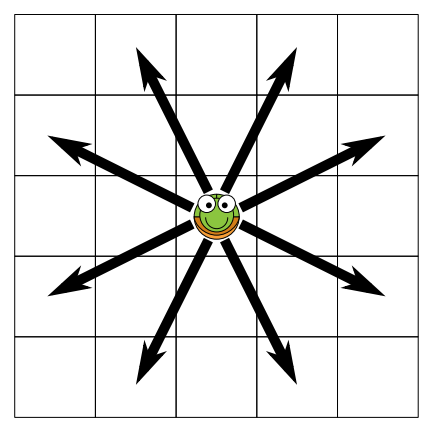
\includegraphics[width = 200px]{problem-image1}
\end{center}

\section*{Vstup a výstup}
Vstup je sestaven s několika testovacích vstupů. Každý řádek vstupu obsahuje 6 čísel na jednom řádku $R$, $C$, $G_R$, $G_C$, $L_R$ a $L_C$. $R$ a $C$ určují velikost (počet řádku a počet sloupců) pole, $1 \leq R, C, \leq 100$. Řehoř nesmí ven z pole, protože to by bylo až moc nebezpečné. $G_R$ a $G_C$ jsou souřadnice (řádek a sloupec) čtverečku, kde se nachází Řehoř, a $L_R$ a $L_C$ jsou souřadnice (řádek a sloupec) vytouženého jetele. $1 \leq G_R, L_R \leq R$, $1 \leq G_C, L_C \leq C$

Pro každý testovací vstup vypište řádek, na kterém bude minimální počet skoků, které potřebuje Řehoř, aby se dostal k jeteli. Není-li možné, aby se Řehoř k jeteli dostal, vypište "impossible".

\section*{Vzorový vstup}
\begin{verbatim}
10 10 10 10 1 1
2 2 1 1 1 2
8 8 1 1 1 2
\end{verbatim}

\section*{Vzorový výstup}
\begin{verbatim}
6
impossible
3
\end{verbatim}

\end{document}
